 \begin{enumerate}
\item Consider one mole of helium gas enclosed in a container at initial pressure \(P_1\) and volume \(V_1\). It expands isothermally to volume \(4V_1\). After this, the gas expands adiabatically and its volume becomes \(32V_1\). The work done by the gas during isothermal and adiabatic expansion processes are \(W_{iso}\) and \(W_{ad}\), respectively. If the ratio \(\frac{W_{iso}}{W_{ad}}=f\ln2\), then find \(\frac{W_{iso}}{W_{ad}}\).
\end{enumerate}

\begin{center}
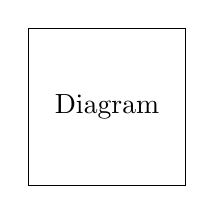
\begin{tikzpicture}
  \node [draw, minimum width=2cm, minimum height=2cm] {Diagram};
\end{tikzpicture}
\end{center}